% Define the document class:
\documentclass[12pt, a4paper, twoside]{report}
%import packages
\usepackage{graphicx} % for images
\usepackage{natbib} % for citation
\bibliographystyle{ctrH} % custom Cite Them Right Harvard referencing
\renewcommand{\bibname}{References} % change name of Bibliography to References
\usepackage{setspace} % allow line spacing to be defined
\onehalfspacing
\usepackage[left=2cm, right=2cm, bottom=2.5cm, top=2cm]{geometry} %define margines
\usepackage{textcomp} % for additional fonts and symbols
\usepackage{tabularx} % for tables
\usepackage{array}
\usepackage{enumitem} % for numbered lists
\usepackage{amssymb} % for additional fonts and symbols
\usepackage{acronym} % for list of acronyms
\usepackage{draftwatermark}
\SetWatermarkText{DRAFT}
\SetWatermarkScale{5}
\raggedbottom

\title{Post-MDT Oncology Workflow Bottlenecks: A Design-Science Study of an NHS Integrated Data Repository and Decision-Support Dashboard to Reduce Delays from MDT Outcome to Treatment Start}
\author{Mark Collins}
\date{\today}

\begin{document}

% Title Page
\begin{titlepage}
    \centering
    {\Large University of Essex Online\par}
    \vspace{1.5cm}
    {\Huge\bfseries Post-MDT Oncology Workflow Bottlenecks: A Design-Science Study of an NHS Integrated Data Repository and Decision-Support Dashboard to Reduce Delays from MDT Outcome to Treatment Start.\par}
    \vspace{2cm}
    {\Large Mark Collins}
    \vfill
    A dissertation dubmitted in partial fulfilment\\
    of the requirements for the degree of\\
    MSc Enterprise IT Management\\
    \vspace{1cm}
    {\large \today\par}
\end{titlepage}

\setcounter{tocdepth}{1}
\tableofcontents

\chapter{Introduction}
Delivering timely cancer care remains a critical priority within the NHS, where delays at any stage of the diagnostic and treatment pathway can negatively affect patient outcomes, experience, and service performance. Recent policy reforms have consolidated the NHS Cancer Waiting Time (CWT) framework into three outcome-focused standards: the 28-day Faster Diagnosis Standard (FDS), the 31-day decision-to-treat to treatment (DTT) standard, and the 62-day referral-to-treatment (RTT) standard—implemented nationally from October 2023 \citep{johnson2024, NHSDigital2026}. These standards place increased emphasis on operational viability, rapid decision-making, and efficient progression of patients through the post-MDT (multidisciplinary team) stages of the oncology pathway. However, many Trusts continue to face systemic challenges in generating timely, accurate, and actionable insights from fragmented data sources.

Within Portsmouth Hospitals University NHS Trust, as in many NHS institutions, key operational data concerning MDT outcomes, clinic scheduling, booking practices, and treatment initiation remain dispersed across siloed systems. Although these systems individually support MDT coordination, outpatient clinic management, and treatment delivery, they lack a consolidated view of pathway performance. This fragmentation makes it difficult for operational managers to detect bottlenecks, identify emerging breach risks, or allocate clinical capacity efficiently. As a result, delays between \textbf{MDT outcomes, first oncology clinic, decision-to-treat}, and \textbf{first definitive treatment} remain insufficiently visible, impairing the Trust's ability to monitor compliance with the 31- and 62-day standards and to respond rapidly to operational pressures.

\section{Problem Statement}

The central problem addressed in this research is the absence of an integrated, operationally focused data infrastructure and decision-support interface to illuminate post-MDT workflow delays and guide timely interventions within an NHS oncology service. Despite the availability of relevant data, the lack of integration and harmonisation across MDT, clinic, and treatment systems results in manual workarounds, inconsistent performance monitoring, and delayed insights. This gap diminishes the ability of operational teams to identify patients at risk of breaching national cancer standards, understand the factors driving variability in pathway intervals, and proactively manage capacity-constrained environments.

Moreover, existing reporting solutions tend to focus on aggregate compliance metrics rather than providing real-time or near–real-time visibility of operational bottlenecks. Without a unified source of truth that aligns event definitions, timestamps, and clinical coding standards \citep{NHSDigital2026}, it becomes difficult to execute performance analysis or support day-to-day decision-making. Literature on Integrated Data Repositories (IDRs) similarly highlights that many institutions struggle with data harmonisation, terminological alignment, and the creation of analytics-ready architectures capable of supporting both research and operational use cases \citep{gagalova2020}.

This study therefore seeks to design, develop, and evaluate a \textbf{lightweight Integrated Data Repository (IDR)} and accompanying \textbf{decision-support dashboard} tailored specifically to the post-MDT oncology workflow. By integrating key pathway events, clinic capacity information, and national standard definitions, the artefact aims to surface bottlenecks, highlight breach risks, and support operational teams in prioritising actions that improve pathway performance.

\section{Research Aim and Objectives}

The overarching aim of this research is to apply Design Science Research (DSR) methods to create and evaluate an IDR-backed dashboard that enhances operational decision-making in post-MDT oncology pathways. The study seeks to generate both a practical artefact—an integrated warehouse plus a usable dashboard—and generalised design knowledge concerning IDR architectures and decision-support principles suitable for NHS operational analytics.

The specific objectives are to:
\begin{enumerate}
    \item \textbf{Analyse and characterise} delays with the post-MDToncology pathway using retrospective data (problem identification).
    \item \textbf{Design} an integrated Data Repository architecture that consolidates and harmonises MDT, clinic scheduling, and treatment data in accordance with national cancer waiting time definitions (design).
    \item \textbf{Develop} a user-centered operational dashboard, informed by ISO 9241-110 usability principles, to surface actionable insights related to pathway bottlenecks and breach risk (development).
    \item \textbf{Demonstrate and evaluate} the artefacts usability, utility, and technical validity through task-based user testing, heuristic evaluation, and metric reconciliation against source systems (evaluation).
    \item \textbf{Abstract and formalise} transferabledesign principles for NHS oncology operational analytics to support future implementations (knowledge contribution).
\end{enumerate}

\section{Design Science Methodology}

This dissertation adopts the Design Science Research (DSR) paradigm, a well-established approach for solving complex, real-world problems through the creation and evaluation of innovative artefacts \citep{hevner2004}. DSR is especially suited to healthcare informatics contexts where organisational, data, and process challenges intersect, and where practical solutions must be both rigorously designed and empirically evaluated.

The research follows the six-activity Design Science Research Methodology (DSRM) proposed by \cite{Peffers2007}:
\begin{enumerate}
    \item \textbf{Problem identification and motivation} – identifying post-MDT workflow delays and the need for integrated information;
    \item \textbf{Define objectives of the solution} – specifying analytic, architectural, and usability requirements for an IDR-backed dashboard;
    \item \textbf{Design and development} – constructing the IDR, data transformation pipelines, and dashboard view;
    \item \textbf{Demonstration} – deploying the artefact with real Trust data to show how it addresses operational problems;
    \item \textbf{Evaluation} – measuring usability, utility, and technical accuracy using multi-method evaluation;
    \item \textbf{Communication} – producing a dissertation delivering both artefact and design knowledge contributions.
\end{enumerate}

This structured methodology ensures that the work moves beyond a local service-improvement project to make a scholarly contribution to the fields of operational analytics, IDR design, and health informatics within NHS settings.

\section{Academic and Practical Significance}

Academically, the research contributes to the limited body of DSR-grounded studies focusing on NHS operational analytics, offering:
\begin{itemize}
    \item an IDR reference architecture for oncology operations;
    \item a set of design principles for NHS-appropriate decision-support dashboards;
    \item an evaluation protocol combining usability metrics, decision-quality testing, and technical verification.
\end{itemize}

Practically, the artefact provides operational teams with a tool that can:
\begin{itemize}
    \item reduce time-to-insight;
    \item support rapid identification of bottlenecks and breach risks;
    \item align capacity planning with demand;
    \item improve pathway monitoring in line with the 28-, 31-, and 62-day standards.
\end{itemize}

Ultimately, the study aims to support faster, more reliable progression from MDT decision to treatment initiation, with the potential to support improved patient care and more effective management of oncology services.
\chapter{Literature Review}

\section{Introduction}

The purpose of this literature review is to synthesise and critically evaluate existing research relevant to the design of an Integrated Data Repository (IDR) and operational analytics dashboard aimed at improving post-MDT oncology pathway efficiency. Timely cancer treatment has profound implications for survival, patient experience, resource utilisation, and system performance. Evidence from national datasets, observational studies, systematic reviews, and informatics research shows that delays between MDT decisions and treatment initiation remain persistent across the NHS. Furthermore, data fragmentation, inconsistent recording practices, and limited visibility of operational bottlenecks hinder the ability of clinicians, MDT coordinators, and service managers to proactively manage these delays.

The review is organised around five interrelated themes:
\begin{enumerate}
    \item MDT operations and evolving pressures on multidisciplinary cancer decision making;
    \item Operational delays across the cancer pathway, particularly diagnosis-to-treatment intervals (DTI);
    \item Data fragmentation and the case for integrated data repositories;
    \item Dashboards and performance-monitoring tools to support operational decision-making;
    \item Emerging data trends and the role of ETL, interoperability, AI and multimodal data integration.
\end{enumerate}

Collectively, this literature forms the conceptual foundation (kernel theory) for the artefact developed in this study. The following sections provide a detailed account of these themes, integrating high-quality evidence from the UK, international datasets, clinical oncology, health informatics, and organisational science.

\subsection{Method}
An iterative literature review was adopted, following the guidance outlined by  \cite{dawson2015} (Figure \ref{fig:LitProc}). An initial search was conducted using Google Scholar and open-access repositories to identify foundationa concepts and terminology related to Integrated Data Repositories, cancer pathways, MDT operations, dashboards, and Design Science Research. These preliminary results infirmed a more structured search strategy applied to ScienceDirect, IEEEXplore, and PubMed.

Searches were limited to peer-reviewed journals, systematic reviews, national audits, and authoritative policy documents published primerily between 2010 and 2026, with earlier seminal works retained where conceptually relevant (e.g. Calman-Hine and Design Science Science foundations). Studies were included if they addressed MDT processes, oncology pathway delays, health data integration, dashboards, usability standards, or operational analytics. Articles focused exclusivly in molecular biology, single-modality clinical trials, or nomn-healthcare data systems were excluded. 

Appoximately 90 sources were reviewed during the processm with around 55 core studies retained for detailed analysis based on relevance, methodological quality, and applicability to NHS operational contexts. Backward citation tracking was used to identify influential seed papers and ensure conceptual completeness.

\begin{figure}
    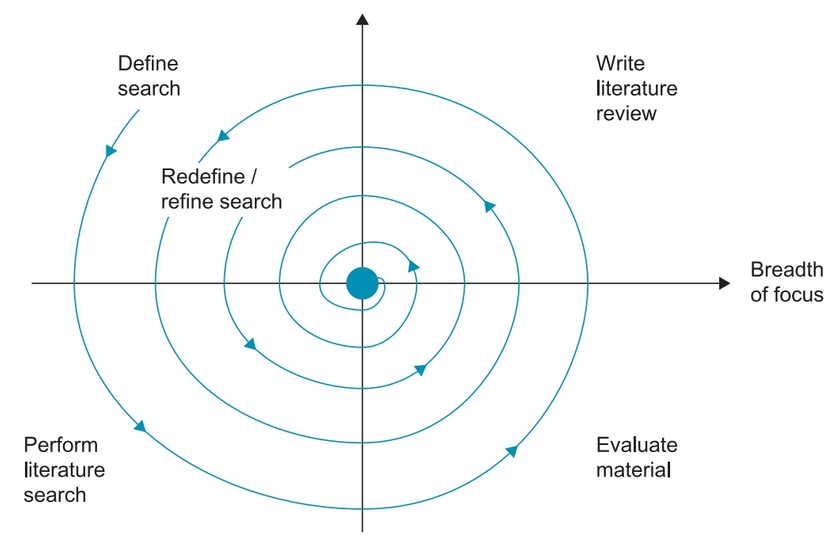
\includegraphics[width=\linewidth]{LitProc.png}
    \caption{Iterative literate review process \citep{dawson2015}}
    \label{fig:LitProc}
\end{figure}

\section{The NHS Cancer Pathway and MDT Framework}

\subsection{MDTs as the Backbone of UK Cancer Care}

Since the publication of the Calman–Hine report and subsequent interventions, MDTs have been embedded as the central governance structure for cancer decision making \citep{haward2006, price2014, morris2006, morris2008}. The MDT model mandates that every new cancer case in the UK is discussed by a multidisciplinary panel including oncologists, surgeons, radiologists, pathologists, specialist nurses, and allied professionals. The 2024 NHS Wales MDT Charter emphasises the crucial role MDTs play in standardising care, reducing unwarranted variation, and improving outcomes by bringing domain experts together in real time \citep{nhswales2024}. Prospective benefits include higher adherence to guidelines, improved communication, shared decision-making, and better coordination of multi-modal treatment plans.

However, the complexity of modern cancer care has increased dramatically alongside rising incidence, new treatment options, biomarker-based stratification, digital imaging volume, and genomic data availability. MDTs now contend with substantially larger case numbers, more complex diagnostic information, and resource pressures that stretch meeting capacity. Professional societies and national audits consistently highlight that MDT meetings are often over-subscribed, under-resourced, and administratively burdensome. These pressures compromise the quality of discussion and create operational bottlenecks that directly affect patient pathways.

\subsection{Evidence of MDT Operational Pressures}

Several studies provide evidence of the challenges affecting MDT functioning:

\begin{itemize}
    \item \cite{soukup2022} conducted a detailed observational analysis of 822 case discussions across three UK MDTs. Administrative and process issues occurred in 30\% of cases, attendance problems in 16\%, and equipment issues in 5\%. These logistical challenges significantly reduced the quality of information and decision-making, demonstrating how operational inefficiencies detract from MDT effectiveness.
    \item \cite{lim2025} analysed 1,488 UK HNC patients across 50 MDTs and found extremely low compliance with national cancer pathway standards: 32.8\% (FDS), 33.3\% (31‑day), and 34.6\% (62‑day). Median DTT-to-treatment was 42 days.
    \item \cite{chakravarty2023} demonstrated that patients referred from secondary-care outpatient pathways experienced significantly longer delays to MDT discussion and treatment (mean 102 vs. 88 days). These patients were also more likely to receive palliative rather than curative treatment.
    \item \cite{law2024} identified a decade of known MDT barriers including time pressures, communication challenges, inconsistent attendance, information deficits, and increasing clinical complexity.
\end{itemize}

While these studies consistently demonstrate operational strain within MDT processes, important limitations remain. Much of the evidence is observational and focuses primarily on decision quality or meeting efficiency rather than downstream operational consequences following MDT outcomes. Moreover, studies such as \cite{soukup2022} and \cite{law2024} emphasise human and organisational factors but do not address how data infrastructure or real-time operational visibility might mitigate these pressures. Large scale cohort analysis (e.g. \cite{lim2025}) quantify non-compliance with national standards but offer limited insights into the specific post-MDT workflow stages where delays emerge. As a result, although MDT pressures are well documented, the mechanisms by which MDT decisions translate into subsequent pathway delays remain poorly illuminated from an operational analytics perspective.  

\subsection{National policy direction and waiting time standards}

NHS England's 2024/25 planning guidance emphasises compliance with the Faster Diagnosis Standard (FDS) and cancer treatment timeliness metrics. Persistent waiting-time challenges, data-quality requirements, and the need for integrated pathway oversight tools are highlighted \citep{parker2026}. Radiotherapy services face particular strain: the Royal College of Radiologists reported over 2,300 breaches of the 31‑day standard in October 2023 \citep{rcr2024}. Hidden waits—such as 20‑week delays between surgery and radiotherapy—are not systematically captured, further illustrating limitations in operational visibility.

\section{Operational Delays in Cancer Pathways}

\subsection{Diagnosis-to-Treatment Interval (DTI) as a Critical Metric}

A robust body of literature demonstrates that prolonged DTI adversely affects survival across multiple cancer types.

Key findings include:

\begin{itemize}
    \item \cite{hanna2020}: A systematic review of 34 studies (1.27M patients) found each four-week delay increased mortality by up to 6–8\% across treatment modalities.
    \item \cite{coca-pelaz2018}: Delays in HNSCC beyond four weeks contribute to tumour progression and reduced local control.
    \item \cite{sharma2016}: Delays greater than 30 days reduce overall survival (HR 1.12), with mortality increasing 2.2\% per additional week.
    \item \cite{villemure-poliquin2025}: Treatment within 30 days improves survival by 9\%.
    \item \cite{saleh2024}: Cervical cancer survival drops dramatically after 30 days.
\end{itemize}

\subsection{Hospital/System Factors Influencing Delay}

Large-scale evidence shows that delays are driven not only by tumour characteristics but also by organisational inefficiencies:

\begin{itemize}
    \item \cite{yun2012}: Delays over one month worsened outcomes, especially in low-volume hospitals.
    \item UK audits (e.g., \cite{lim2025}) highlight delays in biopsies, imaging, scheduling, and treatment booking.
\end{itemize}

\subsection{MDT-specific drivers of post-decision delays}

\begin{itemize}
    \item Missing diagnostic information and administrative errors cause re-discussion delays \citep{soukup2022}.
    \item High caseloads reduce decision completeness.
    \item Secondary‑care referrals introduce additional diagnostic delays \citep{chakravarty2023}.
    \item Capacity constraints (radiotherapy, theatres, oncology clinics) generate downstream bottlenecks.
\end{itemize}

\subsection{Crititcal synthesis of delay literature}
Collectively, the literature provides compelling evidence that prolonged diagnosis-to-treatment intervals adversely affect survival accross multiple cancer types.. However, most studies treat delay as a single agregated interval rather than decomposing it into discrete operational stages. This limits their usefulness for operational improvement, as pathway delays arising from MDT decision latency, clinic availability, scheduling practices, or treatment capacity constraintsare rarely distinguished. Furthermore, while organisational factors such as hospital volume and service configuration are identified as contributors, few studies examine how real-time operational data could be leveraged to predict, prevent, or mitigate delays. This analytical gap constrains the translation of epidemiological evidence into actionable service-level interventions. 

\section{Data Fragmentation and the Need for Integrated Data Repositories}

\subsection{Fragmentation Across NHS Systems}

Oncology data spans EPRs, PAS, pathology, RIS/PACS, radiotherapy systems, chemotherapy e‑prescribing, Somerset/Cosmic, and MDT spreadsheets.

Evidence includes:

\begin{itemize}
    \item Operational policy from Royal Wolverhampton highlights inconsistent event definitions and PTL challenges \citep{theroyalwolverhamptonnhstrust2024}.
    \item \cite{varma2026}: 92.3\% agreement between CWT and hospital data only when treatment occurs within 100 days; discrepancies arise from definition mismatches and missing fields.
\end{itemize}

\subsection{Clinical Data Warehouses (CDWs) and the Evolution Toward IDRs}

Examples:

\begin{itemize}
    \item ROOT CDW: real‑time repository for 67,000+ cancer patients \citep{jung2021}.
    \item ONCO‑FAIR: chemotherapy‑specific FHIR extensions \citep{guilbert2024}.
    \item NHS–industry multimodal genomic-clinical data lake \citep{conway2025}.
    \item HN‑XNAT: federated imaging and radiotherapy repository \citep{butterworth2025}.
\end{itemize}

\subsection{Need for IDRs in NHS Operational Oncology}

Consequences of lacking IDRs include:

\begin{itemize}
    \item inability to track MDT→clinic→treatment transitions,
    \item inconsistent manual workarounds,
    \item reactive rather than proactive breach management,
    \item dependency on retrospective audits.
\end{itemize}

\section{Dashboards, Operational Analytics, and Decision-Support Systems}

\subsection{The Role of Dashboards in Performance Management}

Dashboards synthesise high-volume data for actionable insight. NHS guidance emphasises dashboards as essential for meeting FDS and treatment targets.

\cite{buttigieg2017} identify:

\begin{itemize}
    \item strategic dashboards,
    \item tactical dashboards,
    \item operational dashboards.
\end{itemize}

Key design principles include real‑time refresh, drill‑downs, user-centred design, and integration with data infrastructures.

\subsection{Clinical Decision-Support Dashboards and Multimodal Data}

Examples:

\begin{itemize}
    \item Multimodal CDSS supporting 170,000+ patients, using ETL + NLP + 140 data quality checks \citep{chang2025}.
    \item ROOT CDW: automated ingestion, structured/unstructured data integration \citep{jung2021}.
\end{itemize}

\subsection{Data Quality and Informatics Challenges}

Dashboards depend on strong data foundations:

\begin{itemize}
    \item Coding variation limits dataset reliability \citep{varma2026}.
    \item Oncology workloads require custom FHIR extensions \citep{guilbert2024}.
    \item Multimodal data lakes require governance and standardisation \citep{conway2025}.
\end{itemize}

\section{Usability, HCI, and ISO 9241‑110}

ISO 9241‑110:2020 \citep{internationalorganizationforstandardization2020} provides seven principles:

\begin{enumerate}
    \item Suitability for the task
    \item Self-descriptiveness
    \item Conformity with user expectations
    \item Learnability
    \item Controllability
    \item Error tolerance
    \item Suitability for individualisation
\end{enumerate}

Fraunhofer usability research supports its relevance in healthcare \citep{hunkirchen}.

\section{AI‑Enabled MDT Systems and Emerging Technologies}

Examples include:

\begin{itemize}
    \item EvoMDT: multi-agent MDT recommender reducing decision time by 30–40\% \citep{liu2026}.
    \item TrustedMDT: TNM staging and guideline checking integrated with Teams \citep{soltan2025}.
    \item AI‑MDT for lung cancer: improved throughput and workload reduction \citep{liu2026a}.
    \item AI automation of transcription and summarisation \citep{healthorbit2025}.
    \item Multi-agent consensus MDT system achieving high inter-agent agreement \citep{han2025}.
\end{itemize}

A key insight: AI systems require structured, linked, high‑quality data—yet most NHS operational systems lack it.

\section{Synthesis of Gaps}

The reviewed literature reveals several interlocking gaps that collectively motivate this research. First, despite clear evidence of clinically significant delays between MDT decision and treatment initiation, NHS oncology services lack granular, operationally focused visibility of post-MDT pathway stages. Second, although dashboards are widely promoted as performance management tools, many NHS implementations remain dependent on retrospective, aggregate reporting derived from fragmented and inconsistently defined datasets. As a result, existing dashboards often identify breaches only after they have occurred, limiting their utility for proactive intervention.
Third, while clinical data warehouses and integrated repositories have demonstrated feasibility in research and tertiary settings, their designs typically prioritise longitudinal research use cases rather than real-time operational decision-making. Consequently, issues of event harmonisation, timeliness, and alignment with national cancer waiting time definitions remain unresolved in day-to-day service management. Finally, emerging AI-enabled MDT systems highlight future opportunities for decision automation but simultaneously expose a foundational dependency on structured, integrated, and operationally reliable data infrastructures that are currently absent in most NHS Trusts.
Together, these gaps indicate the need for an artefact that integrates operational oncology data across MDT, clinic, and treatment domains, and presents this information through a user-centred dashboard explicitly designed to support proactive post-MDT workflow management.

\begin{itemize}
    \item \textbf{Gap 1} — Lack of integrated operational visibility
    \item \textbf{Gap 2} — Significant treatment delays persist
    \item \textbf{Gap 3} — Siloed systems hinder analytics
    \item \textbf{Gap 4} — Dashboard capability depends on ETL and interoperability
    \item \textbf{Gap 5} — No integrated framework across MDT, IDR, dashboards, usability
    \item \textbf{Gap 6} — AI MDT systems require structured data not currently available
\end{itemize}

\section{Summary}

This literature review synthesises evidence across MDT functioning, treatment delays, operational workflow challenges, data fragmentation, health informatics, dashboard design, usability standards, and emerging AI-driven MDT tools. MDTs remain vital but increasingly pressured. Delays between diagnosis, MDT decisions, and treatment initiation significantly worsen outcomes, yet Trusts lack the integrated systems required to manage these pathways proactively. Modern CDWs demonstrate feasible architectures, while dashboard and usability literature highlight design imperatives. AI‑enabled MDT systems reveal future potential but highlight the foundational need for high-quality integrated data repositories.

The combined evidence exposes a clear research gap: NHS oncology services require a robust, user-centred, IDR‑backed operational dashboard to improve MDT‑to‑treatment coordination.
\chapter{Methodology}

\section{Overview of Research Design}

This research adopts a Design Science Research (DSR) methodology to address an operational problem in NHS oncology services: the lack of integrated, actionable visibility of delays between MDT outcomes and treatment initiation. DSR is particuarly suitable for this study because it explicitly focuses on the design, construction, and evaluation of an artefact intended to improve a real-world organisational context, while generating transferable design knowledge \citep{hevner2004}.

The primary artefact developed in this study is a lightweight integrated data repository (IDR) ad decision-support dashboard, designed to consolidate post-MDT pathway data and support operational decision-making. In addition to the artefact itself, the research produces a set of evaluated design principles for oncology operational analytics, constituting a contribution to knowledge beyond the local implementation. 

\section{Design Science Research Framework}
The study follows the Design Science Research Methodology (DSRM) proposed by \cite{Peffers2007}, which structures DSR into six interrelated activities. These activities are applied iteratively rather than strictly linearly. 

\subsection{Problem Identification and Motivation}
The problem was identified through:
\begin{itemize}
    \item analysis of NHS Cancer waiting time standards and performance pressures \citep{johnson2024, NHSDigital2026},
    \item eview of literature on MDT operational inefficiencies and pathway delays,
    \item practical experience with Portsmouth Hospitals University NHS Trust.
\end{itemize}
The central problem is the absence of an integrated, operationally focused data infrastructure that aligns MDT outcome, clinic scheduling, and treatment delivery data into a single, trusted view capable of supporting proactive action. 

\subsection{Objectives of a Solution}
The objectives of the solution were derived from both literature synthesis and stakeholder needs, and include:
\begin{itemize}
    \item consolidating post-MDT pathway events into a harmonised, analytics-ready data model;
    \item enabling early identification of patients at risk of breaching the 31- and 62-day standards;
    \item aligning operational risk signals with actionable capacity information;
    \item supporting rapid, routine decision-making through a usable dashboard interface;
    \item complying with NHS data governance and national metric definitions.
\end{itemize}
These objectives directly inform the design principles articulated in Section \ref{DP} and implemented in the artefact.

\subsection{Design and Development}
The design and development activity involved two tightly coupled components:
\begin{enumerate}
    \item Integrated Data Repository (IDR)
    \item Decision-Support Dashboard
\end{enumerate}
The IDR adopts a general-model architecture consisting of a staging layer for ETL and harmonisation, a central warehouse, and an application layer for analytics and visualisation, consistent with IDR literature for single-institution deployments \citep{gagalova2020}.

The dashboard is designed to support operational tasks rather than retrospective reporting, aligning with the role of operational dashboards in healthcare performance management \citep{buttigieg2017}. 

Both components were developed iteratively, guided by explicit design principles derived from prior research and refined during prototyping. 

\subsection{Demonstration}
The artefact is demonstrated using:
\begin{itemize}
    \item retrospective Trust data covering MDT decisions, clinic appointments, and treatment initiation;
    \item realistic operational scenarios reflecting common management tasks (e.g., identifying upcoming breach risks, assessing clinic capacity).
\end{itemize}
Demonstration focuses on illustrating how the artefact supports decision-making that was previously manual, fragmented, or retrospective.

\subsection{Evaluation}
Evaluation is multi-method and aligned with \cite{hevner2004}'s guidance that DSR artefacts must be assessed for utility, quality, and efficacy. Evaluation methods are detailed in Section \ref{EvalStrat}.

\subsection{Communication}
The final activity consists of communicating:
\begin{itemize}
    \item the artefact,
    \item its measured effects, and
    \item the derived design principles,
\end{itemize}
through this dissertation, targeting both academic and and practitioner audiences. 

\section{Research Questions and Method Alignment}

\begin{table}[h]
    \centering
    \begin{tabular}{|p{5cm}|p{3cm}|p{5cm}|}
        \hline
        \textbf{Research Question} & \textbf{DSR Activity} & \textbf{Primary Methods} \\
        \hline\hline
        \textbf{RQ1}: Where do delays occur between MDT outcome and treatment? & Problem identification & Descriptive statistics, interval analysis \\
        \hline
        \textbf{RQ2}: What operational factors predict extended delays? & Problem analysis & Regression and capacity analysis\\
        \hline
        \textbf{RQ3}: Does the artefact improve operational decision-making? & Evaluation & Task-based testing, time-to-answer, accuracy\\
        \hline
        \textbf{RQ4}: What design principles support post-MDT operational analytics? & Design knowledge & Literature synthesis and evaluation synthesis\\
        \hline
    \end{tabular}
    \caption{This mapping ensures methodological coherence between the research questions, artefact, and evaluation.}
    \label{tab:rq-dsr-mapping}
\end{table}

\section{Design Principles} \label{DP}
Design principles represent the design knowledge contribution of this study. They are formulated using a standard DSR structure: \emph{context, intervention}, and \emph{rationale}. These initial principles are refined following evaluation.

\subsection*{DP1: Surface Breach Risks as a Leading Indicator}
If operational teams must prioritise actions in time-constrained cancer pathways, then dashboards should surface leading indicators of breach risk (e.g. days remaining to breach thresholds), because prospective visibility enables earlier and more effective intervention than retrospective compliance metrics. 

\subsection*{DP2: Pair Risk Information with Actionable Capacity Data}
If users are expected to act on identified risks, then risk indicators should be presented alongside relevant capacity and demand information, because risk awareness without visible operational levers does not support decision-making.

\subsection*{DP3: Use Canonical, Standard-Aligned Pathway Events}
If pathway metrics are to be trusted and comparable, then all intervals should be derived from canonical event definitions aligned to NCWTMDS rules, because inconsistent definitions undermine credibility and evaluation validity. 

\subsection*{DP4: Match Data Refresh Cadence to the Action Horizon}
If decisions depend on short operational windows, then data refresh frequency should be aligned to the decision horizon (e.g. daily or near–real-time where feasible), because stale information degrades decision quality.

\subsection*{DP5: Preserve Data Provenance and Auditability}
If analytics are deployed in regulated healthcare environments, then all derived metrics must maintain transparent provenance to source systems, because trust, governance, and reconciliation are essential for adoption.

\subsection*{DP6: Align Interaction Design with Real Operational Tasks}
If dashboards are intended to support complex operational work, then interaction design should reflect users’ real task sequences, because task-aligned interfaces reduce cognitive load and improve decision quality \citep{internationalorganizationforstandardization2020}.

These principles directly inform both the IDR architecture and the dashboard design, and serve as evaluation criteria in Section \ref{EvalStrat}.

\section{Evaluation Strategy} \label{EvalStrat}

Evaluation combines formative and summative methods across four dimensions.

\subsection{Usability Evaluation}
\begin{itemize}
    \item System Usability Scale (SUS)
    \item Heuristic review grounded in ISO 9241-110
    \item Think-aloud walkthroughs
\end{itemize}

\subsection{Utility and Effectiveness}
\begin{itemize}
    \item Task-based experiment with operational users
    \item Primary measures:
    \begin{itemize}
        \item time-to-answer key operational questions,
        \item accuracy of breach-risk identification,
        \item decision quality in constrained scheduling scenarios
    \end{itemize}
\end{itemize}

\subsection{Technical Validity}
\begin{itemize}
    \item Reconciliation of dashboard metrics with source SQL queries
    \item Validation of interval derivations against NCWTMDS rules
\end{itemize}

\subsection{Design Knowledge Evaluation}
\begin{itemize}
    \item Synthesis of user feedback and performance outcomes
    \item Refinement and confirmation of final design principles
\end{itemize}

\section{Ethical and Governance Considerations}
The study operates within UK GDPR and NHS data governance requirements. All data are de-identified or pseudonymised, with access controls and separation between operational and research use. The project follows university ethics procedures and local Trust information governance guidance.

\section{Summary}
This chapter has outlined a rigorous, design-science-based methodology that supports both artefact creation and theory-driven knowledge contribution. By embedding explicit design principles within the DSR framework and evaluating the artefact using multiple complementary methods, the study ensures methodological robustness, practical relevance, and academic contribution.


\addcontentsline{toc}{chapter}{References}
\bibliography{./Project}

\chapter*{List of Acronyms}
\addcontentsline{toc}{chapter}{List of Acronyms}
\begin{acronym}

\acro{AI}{Artificial Intelligence}

\acro{CDSS}{Clinical Decision Support System}
\acro{CDW}{Clinical Data Warehouse}
\acro{CWT}{Cancer Wait Time}

\acro{DSR}{Design Science Research}
\acro{DSRM}{Design Science Research Methodology}
\acro{DTI}{Diagnosis to Treatment Interval}
\acro{DTT}{Decision-to-Treat}

\acro{ETL}{Extract-Transform-Load}
\acro{EPR}{Electronic Patient Record}

\acro{FDS}{Faster Diagnosis Standard}
\acro{FHIR}{Fast Healthcare Interoperability Resources}

\acro{GDPR}{General Data Protection Regulation}

\acro{HCI}{Human Computer Interaction}
\acro{HR}{Hazard Ratio}

\acro{IDR}{Integrated Data Repository}

\acro{JCCO}{Joint Council for Clinical Oncology}
\acro{JSON}{JavaScript Object Notation}

\acro{MDT}{Multidisciplinary Team}

\acro{NCWTMDS}{National Cancer Waiting Times Monitoring Data Set}
\acro{NHS}{National Health Service}

\acro{OIS}{Oncology Information System}

\acro{PAS}{Patient Administration System}
\acro{PACS}{Picture Archiving and Communication System}
\acro{PDCA}{Plan - Do - Check - Act}
\acro{PTL}{Patient Tracking List}

\acro{QA}{Quality Assurance}

\acro{RCR}{Royal College of Radiologists}
\acro{RIS}{Radiology Information System}
\acro{RTT}{Referral To Treatment}

\acro{SABR}{Stereotactic Ablative Body Radiotherapy}
\acro{SACT}{Systemic Anti Cancer Therapy}
\acro{SQL}{Structured Query Language}
\acro{SUS}{System Usability Scale}

\end{acronym}


\end{document}
    